%!TEX root = ../main.tex
% Chapter 4

\chapter{Grundlagen}
\label{Grundlagen}

In diesem Kapitel werden die notwendigen Inhalte, theoretischen Konstrukte und Konzepte erklärt, auf welchen diese Arbeit aufbaut. Zudem wird ein Großteil der Begriffe erläutert, die sich im Glossar und Abkürzungsverzeichnis finden. Während sich Kapitel \ref{Kontext_und_Domaene} auf die sozialen und gesellschaftlichen Merkmale von E-Mails bezog, werden diese im Folgenden hinsichtlich ihrer technischen Merkmale betrachtet. Da die Zielhierarchie die Gewichtung von E-Mails mit einem endlichen Gegenwert vorgibt, beschäftigt sich der zweite Teil dieses Kapitels mit den Mechaniken von \textit{Pay to Win}, welche ein ähnliches Ziel z.B. im Kontext von Videospielen verfolgen.

%----------------------------------------------------------------------------------------

\section{Standards und Technologien zum E-Mail Versand}

E-Mail ist ein asynchrones Kommunikationsmittel im Internet, welches ermöglicht Nachrichten zu versenden \citep[S. 142]{Kurose2014}. Diese Nachrichten sind, in der Ursprungsversion der Technologie, rein text-basiert und können aus beliebigen 7-Bit-\acrshort{ascii} Zeichen bestehen \citep[S. 9]{RFC5322}. E-Mail lässt sich in der Anwendungsschicht des \acrshort{osi}-Referenzmodells verorten, wobei \acrshort{tcp}/\acrshort{ip} durch die zugehörigen Protokolle \acrshort{smtp}, \acrshort{pop3} und \acrshort{imap} verpackt werden.

Als erste Form der E-Mail kann der Befehl \texttt{MAIL} betrachtet werden, welcher 1965 von Noel Morris und Tom van Vleck dem \acrfull{ctss} am \acrshort{mit} hinzugefügt wurde. Das \acrshort{ctss} kann als ein Rechner verstanden werden, welcher verschiedene Benutzerbereiche innerhalb einer Maschine trennt. Nutzer konnten mit dem MAIL-Befehl in einem Terminal Texte an andere Nutzer versenden. Die Texte erschienen im Dateisystem in einer nur dem Empfänger zugänglichen Datei, genannt Mailbox \citep[S. 4]{Vleck2012}. Diese Nachrichten konnten jedoch nur innerhalb des \acrshort{ctss} versendet werden, da der Rechner zu diesem Zeitpunkt noch keine Verbindung an ein externes Netz besaß. 1971 wurde dieses Konzept von Ray Tomlinson aufgegriffen, um Nachrichten über ARPANet, dem Vorläufer des Internets, versenden zu können \citep[S. 4 ff.]{Partridge2008}. Zu diesem Zeitpunkt war das Versenden von Nachrichten betriebssystemabhängig und nicht vereinheitlicht. In \acrshort{rfc} 385 wird die E-Mail erstmals als zusätzliche Funktion von \acrshort{ftp} aufgegriffen und diskutiert \citep[S. 3 f.]{RFC385}. 1982 werden in \acrshort{rfc} 821 eine Systemarchitektur und \acrshort{smtp} erwähnt \citep[S. 2 ff.]{RFC821}. Aus diesem \acrshort{rfc} heraus entwickelten sich die heute üblichen Standards, welche in ihrer aktuellsten Form in \acrshort{rfc} 5321 festgehalten wurden \citep{RFC5321}.

Um Absender und Empfänger eindeutig zu identifizieren, werden E-Mail Adressen verwendet, welche die Struktur \texttt{user@domain.tld} haben (\cite[S. 4 f.]{RFC822}, \cite[S. 2 ff.]{RFC2142}). Der User ist frei wählbar und muss innerhalb einer Domain eindeutig sein. Die Domain entspricht der zugehörigen Adresse des Mailservers samt seiner \acrfull{tld}. Die E-Mail Adresse ist somit eindeutig, wobei keine 1:1-Relation zwischen E-Mail Adressen und Personen oder IP-Adressen besteht.

\begin{figure}[!ht]
	\centering
		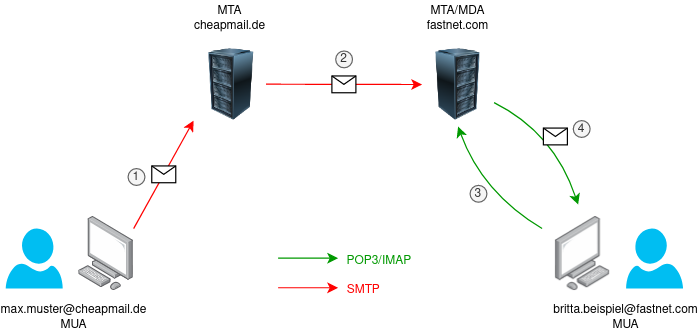
\includegraphics[width=1\textwidth]{Figures/E-Mail Versand.png}
	\caption{Architektur eines E-Mail Versands}
	\label{fig:mail_architektur}
\end{figure}

\noindent Die Struktur des E-Mail Verkehrs entspricht einer Client-Server Architektur und ist in Abbildung \ref{fig:mail_architektur} zu erkennen. Der Client, auch \acrfull{mua} genannt, bietet Möglichkeiten zum Verfassen, Versenden, Empfangen und Verwalten von E-Mails \citep[S. 142 f.]{Kurose2014}. Zum Versand wird das \acrfull{smtp} auf Port 25 (bzw. 587 verschlüsselt) verwendet. \acrshort{smtp} ist ein Protokoll zum Austausch von E-Mails in Netzwerken, verortet auf der Anwendungsschicht im \acrshort{osi}-Modell \citep[S. 4 ff.]{RFC5321}. In einer SMTP-Sitzung werden verschiedene Texte und Statuscodes verwendet, mit denen der MUA mit dem Mailserver, auch \acrfull{mta} kommunizieren kann. 

Zu Beginn der Session kündigt der Client sich mit dem Befehl \texttt{HELO} \\ \texttt{servername.domain.tld} an. Der Server antwortet im Erfolgsfall stets mit dem Statuscode \texttt{250 OK}. Darauf gibt der Client jeweils den Absender mit \texttt{MAIL \\ FROM:<absender@domain.tld>} und den Empfänger mit \texttt{RCPT TO:\\<empfaenger@domain.tld>} an. Zur Übertragung des Nachrichteninhalts wird \texttt{DATA} an den Server gesendet, als Antwort erhält der Client \texttt{354 start mail input} zurück. Nun kann der Client den Inhalt an den Server senden, das Ende wird hierbei durch eine Leerzeile mit einem Punkt folgend dargestellt. Der Server bestätigt erneut mit \texttt{250 OK}, worauf der Client die Verbindung mit \texttt{QUIT} beendet. Der Server quittiert dies zuletzt mit dem Statuscode \texttt{211 closing channel}. Tabelle \ref{tab:smtpversand} zeigt einen beispielhaften Versand einer E-Mail über SMTP von Client zu Server. \citep[S. 4 ff.]{RFC821}

Der Mailserver des Absenders sendet die Nachricht daraufhin an den Mailclient des Empfängers über \acrshort{smtp} weiter. Auch hierbei entspricht der Versand dem in Tabelle \ref{tab:smtpversand} sichtbaren Schema. Der \acrshort{mta} des Empfängers, auch \acrfull{mda} genannt, hält die E-Mail im Postfach des Empfängers vor, bis sich dieser mit seinem Mailserver verbindet. Es ist zu beachten, dass der Empfänger zur Verbindung \emph{\glqq[...] kein SMTP verwenden kann, um die Nachrichten zu erhalten, weil das Abrufen der Nachrichten eine Pull-Operation ist, während SMTP ein Push-Protokoll ist\grqq{}} \citep[S. 150]{Kurose2014}.

\begin{table}[ht]
\centering
\caption[Beispiel: SMTP-Versand einer E-Mail]{Beispielversand einer E-Mail über SMTP}
\begin{tabular}{|l|l|}
\rowcolor{red!25}
\hline
\textbf{Client}                                                                                                                                                                                                                           & \textbf{Server}      \\ \hline
\texttt{HELO smtp.eme.fr}                                                                                                                                                                                                                          & \texttt{250 OK}               \\ \hline
\texttt{MAIL FROM:jean-bob@eme.fr}                                                                                                                                                                                                                 & \texttt{250 OK}               \\ \hline
\texttt{RCPT TO:billy@yahoo.co.uk}                                                                                                                                                                                                                 & \texttt{250 OK}              \\ \hline
\texttt{DATA}                                                                                                                                                                                                                                    & \texttt{354 start mail input} \\ \hline
\begin{tabular}[c]{@{}l@{}}From: \textless{}jean-bob@eme.fr\textgreater\\ To: \textless{}billy@yahoo.co.uk\textgreater\\ Subject: Cake\\ Date: Thu, 7 Apr 2022 16:26:49 +0200\\ \\ Hello Billy, how do you like my cake?\\ .\end{tabular} & \texttt{250 OK}              \\ \hline
\texttt{QUIT}                                                                                                                                                                                                                                      & \texttt{211 closing channel}  \\ \hline
\end{tabular}
\label{tab:smtpversand}
\end{table}

\noindent Aus diesem Grund wurden das \acrfull{pop3} und das \acrfull{imap} entworfen, welche \acrshort{mua}s den Abruf von E-Mails ermöglichen. \acrshort{pop3} kommuniziert über Port 110 (bzw. 995 verschlüsselt) und besitzt nur eingeschränkte Funktionen. Nach einem Verbindungsaufbau werden drei Phasen durchlaufen: Autorisierung, Transaktion und Aktualisierung. Zur Autorisierung überträgt der Client jeweils seinen User mit \texttt{USER} und sein Passwort mit \texttt{PASS} im Klartext und erhält bei erfolgreicher Autorisierung \texttt{+OK} als Statusmeldung zurück. In der Transaktionsphase kann der Client den Status des Postfachs mit \texttt{STAT}, eine Liste der E-Mails mit Größe mit \texttt{LIST} und den Inhalt einzelner E-Mails mit \texttt{RETR} abrufen. Bei letztem Befehl wird die Nummer der E-Mail im Postfach mit angegeben, die beim Aufruf von \texttt{LIST} angezeigt wird. Mit der selbigen Nummer ist es auch möglich E-Mails vom Server zu löschen indem man \texttt{DELE} nutzt. Hierbei wird das Löschen nicht direkt ausgeführt. Stattdessen beendet der Client die Sitzung mit \texttt{QUIT}, woraufhin die Aktualisierungsphase gestartet und alle \texttt{DELE}-Befehle ausgeführt werden. Um Löschungen vor Sitzungsende abzubrechen, kann \texttt{RSET} verwendet werden. Der beispielhafte Abruf der E-Mail aus Tabelle \ref{tab:smtpversand} ist in Tabelle \ref{tab:pop3abruf} zu sehen. \citep[S. 3 ff.]{RFC1939}


\begin{table}[ht]
\centering
\caption[Beispiel: POP3-Abruf einer E-Mail]{Beispielabruf der E-Mail aus Tabelle \ref{tab:smtpversand} mit POP3}
\begin{tabular}{|l|l|}
\rowcolor{red!25}
\hline
\textbf{Client} & \textbf{Server}                                                                                                                                                                                                                      \\ \hline
\texttt{USER billy@yahoo.co.uk}            & \texttt{+OK}                                                                                                                                                                                                                                  \\ \hline
\texttt{PASS secret-passwort}          & \texttt{+OK}                                                                                                                                                                                                                                  \\ \hline
\texttt{LIST}            & \begin{tabular}[c]{@{}l@{}}\texttt{+OK 1 37}\\ \texttt{+OK 2 534}\end{tabular}                                                                                                                                                                        \\ \hline
\texttt{RETR 1}          & \begin{tabular}[c]{@{}l@{}}From: \textless{}jean-bob@eme.fr\textgreater\\ To: \textless{}billy@yahoo.co.uk\textgreater\\ Subject: Cake\\ Date: Thu, 7 Apr 16:26:49 +0200\\ \\ Hello Billy, how do you like my cake?\\ .\end{tabular} \\ \hline
\texttt{DELE 1}          & \texttt{+OK}                                                                                                                                                                                                                                  \\ \hline
\texttt{QUIT}            & \texttt{+OK}                                                                                                                                                                                                                                  \\ \hline
\end{tabular}
\label{tab:pop3abruf}
\end{table}

Da \acrshort{pop3} E-Mails lediglich abrufen und löschen kann, wurde \acrshort{imap} entworfen, welches die Funktionalitäten von \acrshort{pop3} erweitert und dadurch die Komplexität des Abrufs erhöht. \acrshort{imap} bietet die Möglichkeit verschiedene Ordner zu erstellen und zu verwalten, darüber hinaus können E-Mails in einer gekürzten Form abgerufen werden. Letzteres ist insbesondere bei Clients mit schwacher Internetverbindung hilfreich, da der Nutzer einen Überblick enthält und sich dann entscheiden kann, welche Nachricht er laden will. \citep[S. 2 ff.]{RFC3501}


\begin{table}[]
\centering
\caption[Beispiel: IMAP-Abruf einer E-Mail]{Beispielabruf der E-Mail aus Tabelle \ref{tab:smtpversand} mit IMAP}
\begin{tabular}{|l|l|}
\rowcolor{red!25}
\hline
\textbf{Client}                             & \textbf{Server}                                                                                                                                                                                                                                 \\ \hline
\texttt{a001 LOGIN billy secret-passwort}            & \texttt{a001 OK LOGIN}                                                                                                                                                                                                                                   \\ \hline
\texttt{a002 SELECT INBOX}                           & \begin{tabular}[c]{@{}l@{}}* \texttt{2 EXISTS}\\ * \texttt{FLAGS} \texttt{(\textbackslash{}Answered \textbackslash{}Deleted \textbackslash{}Seen)}\\ * \texttt{OK {[}UNSEEN 1{]}}\\ \texttt{a002 OK {[}READ-WRITE{]} SELECT}\end{tabular}      \\ \hline
\texttt{a004 FETCH 1 BODY{[}HEADER{]}}               & \begin{tabular}[c]{@{}l@{}}* \texttt{1 FETCH (BODY{[}HEADER{]}}\\   From: \textless{}jean-bob@eme.fr\textgreater\\   To: \textless{}billy@yahoo.co.uk\textgreater\\   Subject: Cake\\   Date: Thu, 7 Apr 16:26:49 +0200\\ \texttt{)}\\ \texttt{a004 OK FETCH}\end{tabular} \\ \hline
\texttt{a005 FETCH 1 BODY{[}TEXT{]}}                 & \begin{tabular}[c]{@{}l@{}}* \texttt{1 FETCH (BODY{[}TEXT{]}}\\   Hello Billy, how do you like my cake?\\ \texttt{)}\\ \texttt{a005 OK FETCH}\end{tabular}                                                                                                                 \\ \hline
\texttt{a006 STORE 1 +FLAGS \textbackslash{}Deleted} & \texttt{a006 OK +FLAGS}                                                                                                                                                                                                                                  \\ \hline
\texttt{a007 EXPUNGE}                                & \begin{tabular}[c]{@{}l@{}}* \texttt{1 EXPUNGE}\\ \texttt{a007 OK EXPUNGE}\end{tabular}                                                                                                                                                                           \\ \hline
\texttt{a008 LOGOUT}                                 & \texttt{a008 OK LOGOUT}  \\ \hline
\end{tabular}
\label{tab:imapabruf}
\end{table}

Tabelle \ref{tab:imapabruf} zeigt den Abruf der E-Mail aus Tabelle \ref{tab:smtpversand}. Zum Verbindungsaufbau wird der Befehl \texttt{LOGIN} mit User und Passwort in Klartext verwendet. Der Server antwortet mit \texttt{OK}, gefolgt vom Befehlsnamen, in diesem Fall \texttt{OK LOGIN}. Hierbei besitzt jeder Befehl ein vorangehendes Tag, anhand welchem sich ein Befehl zuordnen lässt, beispielsweise \texttt{a001}, \texttt{a002}... \citep[S. 6 f.]{RFC3501}. Nach erfolgreicher Autorisierung kann der Client verschiedene Ordner öffnen, zum Beispiel den Posteingang mit \texttt{SELECT INBOX}. Er erhält sowohl ein \texttt{OK} vom Server, als auch eine Liste der im Ordner liegenden E-Mails, die erste ungelesene E-Mail, sowie die verfügbaren Flags, die die E-Mails weiter klassifizieren. Ähnlich zu \texttt{RETR} kann mit \texttt{FETCH} der Inhalt einer E-Mail angezeigt werden. Hierbei können sowohl der Nachrichten-Header als auch der Body angezeigt werden mit \texttt{FETCH BODY[HEADER]}, bzw. \texttt{FETCH BODY[TEXT]}. Der Aufbau einer E-Mail wird nachfolgend detaillierter erläutert. Zum Löschen wird \texttt{STORE +FLAGS \textbackslash Deleted} ausgeführt, wodurch eine Nachricht entsprechend markiert wird. Um diese Nachrichten zu entfernen, wird \texttt{EXPUNGE} verwendet. Hierbei werden markierte Nachrichten permanent gelöscht. Abschließend kann der Client die Verbindung mit \texttt{LOGOUT} trennen. \citep[S. 2 ff.]{RFC3501}

Das zuvor beschriebene Szenario deckt jedoch nur den Erfolgsfall ab. Es ist jedoch möglich, dass ein Mailserver nicht erreichbar ist. Ist der \acrshort{mta} des Absenders nicht erreichbar, hält der \acrshort{mua} die Nachricht in einer Warteschlange vor und versucht sie erneut zu versenden. Selbiges gilt für einen \acrshort{mta}, der versucht die Nachricht an den \acrshort{mda} weiterzuleiten. Kann die Nachricht nach wiederholten Versuchen in festlegten Intervallen nicht versendet werden, wird sie aus der Nachrichtenwarteschlange entfernt und der Absender wird über den Vorgang informiert \citep[S. 144 f.]{Kurose2014}. Bei den Abrufprotokollen \acrshort{pop3} und \acrshort{imap} wird der Nutzer direkt informiert, wenn sein \acrshort{mda} nicht verfügbar ist, wiederholte Versuche müssen selbst initiiert werden.

E-Mails besitzen ein bestimmtes Format, welches in \acrshort{rfc} 5322 definiert wurde. Unterteilt wird in einen Header, der alle notwendigen Metainformationen enthält, und einen Body, der den eigentlichen Nachrichteninhalt enthält \citep[S. 6 ff.]{RFC5322}. Dabei sind Header und Body (auch Payload genannt) von einer Leerzeile getrennt, um sie auseinander zu halten. Zeile 6 in Tabelle \ref{tab:smtpversand} zeigt ein entsprechendes Beispiel. Verpflichtend sind dabei lediglich der Absender, mit \texttt{From:} spezifiziert, der Empfänger, mit \texttt{To:} spezifiziert und das Datum der Nachricht, mit \texttt{Date:} spezifiziert \citep[S. 18]{RFC5322}. Darüber hinaus existieren weitere standardisierte Header-Felder, wie z.B. \texttt{Priority} für die Priorität einer E-Mail.  Es ist außerdem möglich eigene Header zu setzen, wenn diese mit einem \texttt{X-} beginnen \citep[S. 24]{RFC822}. 

Für Header und Body stehen in der Ursprungsform der E-Mail lediglich 7-Bit \acrshort{ascii}-Zeichen zur Verfügung. Um diese Beschränkungen aufzuheben, wurden in \acrshort{rfc} 2045 Erweiterungen, \acrfull{mime} genannt, eingeführt. \acrshort{mime} bieten die Möglichkeit verschiedene Zeichensätze zu verwenden, indem diese in \acrshort{ascii} umkodiert werden \citep[S. 3 f.]{RFC2045}. Hierzu werden drei neue Headerfelder genutzt, welche die MIME-Version (\texttt{MIME-Version}), den Inhaltstyp (\texttt{Content-Type}) und die Kodierung (\texttt{Content-Transfer-Encoding}) definieren. Als MIME-Version wird 1.0 angegeben, als Content-Type können verschiedene Typen angegeben werden, die der jeweilige \acrshort{mua} selbst interpretiert. Mögliche Inhaltstypen sind unter anderem \texttt{text/plain} für einfachen Text, \texttt{text/html} für E-Mails im Markup-Format mit Styling, \texttt{image/png} für Bilder im \acrshort{png}-Format. Bei \acrshort{html} ist zu beachten, dass sich die Interpretation je nach \acrshort{mua} unterscheiden kann, wodurch unterschiedliche Darstellungen der selben Nachricht möglich sind \citep[S. 6 f.]{RFC2046}. Zum Versenden von Anhängen zusätzlich zu einer Nachricht wird \texttt{multipart/mixed} angegeben, wobei die einzelnen Anhänge durch einen \texttt{boundary}-Eintrag voneinander getrennt werden. Diese Einträge enthalten jeweils einen eigenen \texttt{Content-Type} und können weitere Informationen wie einen Dateinamen enthalten \citep[S. 268 f.]{Zisler2014}. 

Zuvor wurde bereits erläutert, wie ein Absender informiert wird, wenn seine Nachricht nicht an den \acrshort{mda} des Empfängers weitergeleitet werden kann. Es ist jedoch auch möglich eine Zustellbestätigung zu erhalten. Sowohl die Bestätigung über eine erfolgreiche als auch eine fehlgeschlagene Zustellung wird \acrfull{dsn} genannt. Diese werden über \acrshort{smtp} versendet, wobei als Absender \texttt{MAILER-DAEMON@domain.tld} und als Empfänger \texttt{<>} im Header angegeben wird \citep[S. 19 ff.]{RFC3461}. Zusätzlich wird über das Feld \texttt{Diagnostic-Code} ein Statuscode zurückgegeben, wie z.B. \texttt{5.2.2} bei einem vollen Posteingang des Empfängers oder \texttt{5.3.4} bei einer Nachricht, die zu groß für einen Mailserver ist \citep[S. 7 ff.]{RFC3463}. Da die Zustellbestätigung lediglich den Erhalt der E-Mail des \acrshort{mda} zusichert, wurden mit RFC 8098 und RFC 3503 Empfangsbestätigungen, auch \acrfull{mdn} genannt, eingeführt. Diese Bestätigungen werden vom jeweiligen \acrshort{mua} über \acrshort{pop3} oder \acrshort{imap} versendet, wenn er eine E-Mail erhalten hat \citep[S. 3 f.]{RFC3503}. Ob diese auch vom Empfänger gelesen wurde, ist dabei irrelevant \citep[S. 30 f.]{RFC8098}.

Ein großes Problem von E-Mails stellt die Sicherheit dar. So übertragen die vorgestellten Protokolle sowohl die Nachrichten als auch die Nutzeranmeldedaten im Klartext. Um letzteres abzusichern, kann das \acrfull{tls} Protokoll verwendet werden. Mit \acrshort{tls} können Daten im Internet verschlüsselt übertragen werden, wobei der Diffie-Hellman-Schlüsselaustausch verwendet wird, welcher private und öffentliche Schlüsselpaare kombiniert \citep[S. 95 f.]{RFC8446}. Um den Nachrichteninhalt selbst zu verschlüsseln oder zu signieren, bieten sich \acrfull{smime} an. Hierzu benötigen Empfänger ein von einer \acrfull{ca} ausgestelltes Zertifikat in Verbindung mit einem privaten Schlüssel; Absender benötigen zudem das Zertifikat des Empfängers \citep[S. 5 ff.]{RFC8551}. Mit diesen Informationen kann ein Absender eine E-Mail verschlüsseln und/oder signieren. Hierzu wird der Content-Type \texttt{multipart/signed} verwendet, wobei der erste Teil den Nachrichteninhalt und der zweite Teil Informationen zur Signatur in einer .p7s-Datei enthält \citep[S. 30 ff.]{RFC8551}. Mit Hilfe dessen kann der Empfänger die Echtheit und Authentizität der Nachricht prüfen. Aufgrund des mit diesem Verfahren verbundenen Aufwandes (Beschaffung eines Zertifikats bei einer \acrshort{ca}), wird \acrshort{smime} bei privaten Nutzern wenig verwendet, während es in Unternehmen häufig zu internen Signierung und Verschlüsselung angewendet wird \citep[S. 266]{Kappes2013}.


%----------------------------------------------------------------------------------------

\section{Bezahlsysteme zur Schaffung von Vorteilen in Videospielen (Pay to Win)}
\label{Bezahlsysteme_zur_Schaffung_von_Vorteilen_in_Videospielen_(Pay_to_Win)}

Die Priorisierung von E-Mails mittels eines Gegenwertes ähnelt dem Prinzip von Bezahlsystemen zur Schaffung von Vorteilen in Videospielen, auch Pay to Win oder Pay2Win genannt. Pay to Win beschreibt die Monetarisierung von Videospielen, die kostenlos oder kostenpflichtig sind. Bei der Monetarisierung handelt es sich um Mikrotransaktionen, die innerhalb der Spielwelt geschehen und damit keine feste Grenze zum Spielgeschehen aufweisen \citep[S. 18]{Tomic2019}. Pay2Win grenzt sich dabei von anderen Mikrotransaktionen ab, da es einen direkten Einfluss auf den Erfolg des Spielers hat, wohingegen kaufbare kosmetische Elemente den Erfolg des Spielers nicht beeinflussen \citep[S. 124 f.]{Reza2019}. Besonders in kostenlosen Spielen, verstärkt im mobilen Bereich, wird Pay2Win verwendet um Umsatz zu erzeugen. Hierbei werden Spieler nach einer gewissen Spielzeit kostenpflichtige Objekte und Aktionen angeboten, um ihren Fortschritt zu beschleunigen. Der Vorteil dieses Vorgehens ist, dass das Preismodell auf jeden Nutzer individuell zugeschnitten werden kann, was die Wahrscheinlichkeit einer Transaktion erhöht \citep[S. 2]{Alha2014}.

Grundsätzlich können zwischen drei Arten von Transaktionen unterschieden werden. So können gewisse Objekte in einem Spiel durch eine einmalige Zahlung erworben werden und bleiben dauerhaft im Besitz des Spielers. Hierbei handelt es sich nur um Pay2Win, wenn die Objekte dem Spieler einen Vorteil verschaffen. Eine weitere Art der Transaktionen sind Abonnements, bei denen Spieler einen temporären Vorteil erkaufen, der nur für die Zeit des Abonnements gilt. Die am weitesten verbreitete Art der Transaktion sind sogenannte Lootboxen. Lootboxen sind Pakete, welche Spieler kaufen können, um neue Objekte zu erhalten, wobei sie nicht wissen welche Objekte sie erhalten und welchen Wert diese widerspiegeln \citep[S. 20]{Tomic2019}. Spieler haben dabei keinen Einfluss auf den Inhalt von Lootboxen.

Die Effekte von Pay2Win unterscheiden sich je nach Art des Spiels. So dienen Transaktionen in einem Einzelspieler-Modus dem individuellen Fortschritt, beziehungsweise der Erleichterung des Spielers. In Mehrspieler-Modi hingegen erzeugt Pay2Win eine Ungleichheit zwischen Spielern, da die Zahlenden bevorzugt werden. Während diese Mechanik anfangs nur in kostenlosen Spielen auftrat, wird sie mittlerweile auch verstärkt in Titeln angewendet, die ohnehin kostenpflichtig sind \citep[S. 19]{Tomic2019}.

Die Definition eines Pay2Win-Spiels ist nicht klar definiert und von subjektiven Bewertungen geprägt. Aus diesem Grund versuchen \cite{Tregel2020} in einer Befragung Kriterien zu erarbeiten, welche ein Spiel als Pay2Win deklarieren. Es wurden 13 Kriterien erarbeitet, von denen fünf eine Zustimmung von über 2/3 der Befragten erhielten. Ein Spiel kann als Pay2Win erachtet werden, wenn es ab einem Punkt kaum/nicht mehr möglich ist es ohne Zahlung fortzuführen oder Fortschritt zu erlangen. Außerdem wurden Objekte, die einen Vorteil verschaffen und nur mit Echtgeld gekauft werden können, aufgeführt. Dies ist insbesondere ein Indikator von Pay2Win, wenn diese Objekte einen permanenten Vorteil verschafften oder in einem Mehrspieler-Modus hilfreich sind \citep[S. 179]{Tregel2020}. Nicht alle Kriterien müssen auf ein Spiel zutreffen, damit es als Pay2Win gilt.

Der größte Kritikpunkt an Pay2Win ist, abgesehen von der bereits erwähnten Privilegierung, der Einfluss, den Mikrotransaktionen auf Spieler haben. Insbesondere bei Lootboxen, deren Inhalt für den Spieler nicht vorhersehbar ist, finden sich Parallelen zum Glücksspiel. Da das eigene Geld meist in spielinterne Währung umgetauscht werden muss, deren Wechselkurs nicht transparent dargestellt wird, können Lootboxen mit Glücksspiel in Kasinos verglichen werden, in denen Chips o.ä. gekauft werden müssen, um teilzunehmen (\cite[S. 7 ff.]{Drummond2018},, \cite[S. 185 ff.]{Nielsen2019}). Da die Lootboxen direkt in das Spielgeschehen integriert werden, werden die Zahlungen von den Spielern seltener hinterfragt. Das führt insbesondere dazu, dass Menschen, die ein höheres Risiko haben von Glücksspiel abhängig zu werden, auch größere Summen in Lootboxen investieren \citep[S. 5 f.]{Zendle2018}. Darüber hinaus können auch Minderjährige, die keinen Zugang zu konventionellem Glücksspiel haben und tendenziell anfällig für jenes sind, Lootboxen kaufen. Dieser Umstand wird dadurch deutlicher, dass ein Großteil des Einkommens der Spieleentwickler durch Lootboxen von einer kleinen Spielergruppe kommt (\cite[S. 8 f.]{Zendle2020},, \cite{Takahashi2014}). Diese Spieler sind oft nicht in der finanziellen Position ihre Käufe zu tätigen und fallen den Mechaniken von Pay2Win zum Opfer \citep{Close2021}. Ein weiterer Indikator dafür, dass Lootboxen mit Glücksspiel verglichen werden können, sind die Verhaltensweisen von Spielern, die sich mit Glücksspielern überschneiden. So fanden verschiedene Studien heraus, dass Käufer von Lootboxen ihr eigentliches Budget überschreiten, um einen Einsatz zurück zu gewinnen; ein Indikator für mal-adaptives Verhalten (\cite[S. 9 ff.]{Nielsen2019},, \cite[S. 1968 f.]{King2018a},, \cite[S. 4 f.]{Xiao2021}).

Um die Problematik von Pay2Win und insbesondere ihre Auswirkungen hinsichtlich Spielsucht und ethischer Aspekte abzumildern, schlagen \cite{King2018} verschiedene Maßnahmen vor, die mit sozialer Verantwortung der Softwareentwickler einhergehen. Diese Maßnahmen sind in vier Kategorien verortet, die im Folgenden erläutert werden. Die erste Kategorie beschäftigt sich mit dem Design und dem Prozess von Mikrotransaktionen in Spielen. Hierbei wird die Art und Weise wie Objekte gekauft werden können adressiert. So sollen Spieler Preise stets in echter Währung einsehen können und ein Limit setzen, wie viel Geld sie in einem bestimmten Zeitraum ausgeben wollen. Außerdem soll der Zahlungsprozess durch Pausen und das Eingeben der Anmeldedaten verlangsamt werden, sodass Spieler reflektieren können, ob sie ein Objekt wirklich kaufen wollen. Lootboxen sollen außerdem nur Objekte enthalten, die Spieler auch innerhalb des Spiels erhalten können, zudem dürfen diese nicht ablaufen. Die Privilegierung von Spielern soll ebenfalls nicht möglich sein, sodass eine gewisse Fairness in Mehrspieler-Modi gewährleistet ist. Zudem darf der Kauf von Lootboxen nicht künstlich hervorgehoben werden durch zeitlich begrenzte Angebote, besondere Animationen oder andere Einfluss nehmende Strategien. Die zweite Kategorie behandelt die Transparenz von Features. Hierbei sind Entwickler angehalten Lootboxen als Teil des Spiels schon beim Verkauf zu deklarieren und die Chancen zum Erwerb von gewissen Objekten in Lootboxen zu kommunizieren. Als dritte Kategorie wird der Verbraucherschutz angeführt. Spiele mit Lootboxen, bzw. der Kauf von Lootboxen soll mit einer Altersbeschränkungen versehen werden. Außerdem sollen Spieler ihre bisherigen Zahlungen einsehen und limitieren können, analog zu Sportwetten. Eine Checkliste für die problematisches Verhalten soll Spielern helfen ihren Umgang mit Lootboxen zu bewerten. Zuletzt befasst sich die Kategorie der Verbraucherinformation und Industrieverantwortung mit der Informationen über Änderungen am Pay2Win-System, sowie der proaktiven Information der Spieler zu gesundem Glücksspiel \citep[S. 169 ff.]{King2018}. Auch wenn diese Vorschläge die Mechanik von Pay2Win spielerfreundlicher und sicherer machen würden, kann nicht davon ausgegangen werden, dass sie implementiert werden, wenn es keine Verpflichtung, beispielsweise durch den Gesetzgeber, gibt.

Als Beispiel für den Einsatz von Pay2Win eignet sich der Spielmodus \textit{FIFA Ultimate Team} der Spielreihe \textit{FIFA} von EA Sports. In diesem Mehrspieler-Modus stellen Spieler eine eigene Mannschaft aus Fußballprofis zusammen. Diese Profis haben dabei verschiedene Attribute, wie z.B. \textit{Sprintgeschwindigkeit} oder \textit{Schusskraft}, die mit Werten von 1 bis 100 beschrieben werden. Je höher ein Attribut ist, desto besser ist der Profi. Spieler können in Turnieren und Ligen Münzen gewinnen, mit welchen sie Profis auf Auktionen kaufen können. Zusätzlich gibt es die Möglichkeit Pakete zu kaufen, in denen sich, analog zu Sammelkarten, Profis befinden können, wobei der Spieler nicht weiß, welche Profis er erhält. Diese Pakete können ebenfalls mit Echtgeld gekauft werden und erfüllen somit die Kriterien für eine Lootbox. Hierbei werden die Pakete nicht direkt gekauft, stattdessen wird das Geld in sogenannte \textit{FIFA Points} umgewandelt, mit welchen man wiederum die Lootboxen kaufen kann. Zwar ist es auch möglich Pakete mit Münzen zu kaufen, in der Regel spiegelt der Aufwand für den Spieler den Ertrag des Paketes nicht wieder \citep[S. 188]{Tregel2020}. So wurden für das Finalturnier der FIFA eSports Meisterschaften 2019 ca. 27.000\$ benötigt, um mit Pay2Win ein ausreichendes Team zu stellen \citep{Akerman2019}.